\chapter{Matematik}
\label{cha:matematik}

I dette appendiks skal vi indføre nogle nyttige matematiske redskaber,
der er essentielle for fysikken. Selvom du måske kender noget af
matematikken i forvejen, så anbefaler vi alligevel kraftigt, at du
læser appendikset, fordi vi sandsynligvis præsenterer det på en anden
måde, end du er vant til fra gymnasiet.

\section{Polære Koordinater, Cosinus og Sinus}
Forestil dig en lille kugle for enden af en snor, der roterer rundt i
en cirkelbevægelse som på tegningen nedenfor.
\begin{center}
	\begin{tikzpicture}[scale=.8]
	\draw [->] (-3.2,0) -- (3.2,0);
	\draw [->] (0,-3.2) -- (0,3.2);
	\draw (0,0) circle (2.4);
	\draw (0,0) -- (1.49186,1.87998);
	\draw [fill] (1.49186,1.87998) circle (.07);
	\draw [dashed] (1.49186,1.87998) -- (1.49186,0);
	\draw [dashed] (1.49186,1.87998) -- (0,1.87998);
	\node [right] at (3.2,0) {$x$};
	\node [above] at (0,3.2) {$y$};
	\node at (1.17*1.49186,1.17*1.87998) {$P$};
	\node [below] at (1.49186,0) {$x$};
	\node [left] at (0,1.87998) {$y$};
	\draw [->] (1.2*.4,0) to[out=70, in=-25] (1.2*.2486,1.2*.3133);
	\node at (.7,.4) {$\theta$};
	\node [above,rotate=51] at (.5*1.49186,.5*1.87998) {$r$};
	\node [right] at (3,2.5) {$x = r \cos\theta$};
	\node [right] at (3,1.8) {$y = r \sin\theta$};
	\end{tikzpicture}
\end{center}
Kuglen roterer rundt i et to-dimensionelt plan. Lad os sige, at til et
bestemt tidspunkt befinder kuglen sig i punktet $P$. Når vi har lagt
et koordinatsystem som på tegningen kan vi beskrive punket $P$ ved at
angive dets $x$-værdi og $y$-værdi. Disse koordinater ($x$ og $y$)
kaldes \emph{kartesiske} koordinater. Det er muligt at beskrive $P$
ved hjælp af andre koordinater, fx er det i dette tilfælde smart at
beskrive $P$ ved at angive afstanden $r$ fra centrum (origo) og
vinklen $\theta$ mellem $x$-aksen og linjen fra origo til $P$, se
tegningen. Disse koordinater ($r$ og $\theta$) kaldes \emph{polære}
koordinater.

Fordelen ved polære koordinater er tydelig, når vi tænker
på en kugle i en snor, der roterer rundt: Til et senere tidspunkt har
kuglen flyttet sig til et andet punkt på cirklen. I kartesiske
koordinater vil det nye punkt have både en ny $x$- og $y$-værdi, men i
polære koordinater vil vinklen $\theta$ være ny, men radius $r$ er
uændret. Så i polære koordinater er det altså kun én koordinat, der
ændres, når kuglen roterer rundt, hvilket er nemmere at arbejde med end
to, der ændrer sig.

Relationerne mellem kartesiske og polære koordinater er:
\begin{equation} \label{eq:kartesisk/polaer}
\begin{aligned}
x &= r \cos \theta \\
y &= r \sin \theta \\
r &= \sqrt{x^2 + y^2} \\
\theta &= \arctan (y/x) \; ,
\end{aligned}
\end{equation}
hvor $\arctan$ er den inverse funktion til tangens, men udtrykket for
$\theta$ vil I ikke få brug for. I udtrykkene for $x$ og $y$ indgår
henholdsvis funktionerne cosinus og sinus. De er 
defineret som på tegningen: Hvis $\theta$ angiver vinklen mellem
$x$-aksen og et punkt, så er
\begin{align*}
&\cos \theta = \text{$x$-koordinaten for punktet på cirklen med
	radius $1$}\\
&\sin \theta = \text{$y$-koordinaten for punktet på cirklen med
	radius $1$}
\end{align*}
Cosinus og sinus har også noget med trekanter at gøre. Hvis vi kigger
på tegningen af cirklen igen, ser vi, at den indeholder to retvinklede
trekanter: $OxP$ og $OyP$, hvor $O$ betegner centrum. I de to
trekanter er hypotenusen $r$, og de to sidelænger er $x = r
\cos\theta$ og $y = r \cos\theta$. Vi kan altså lave følgende tegning,
der illustrerer længderne i en retvinklet trekant:
\begin{center}
	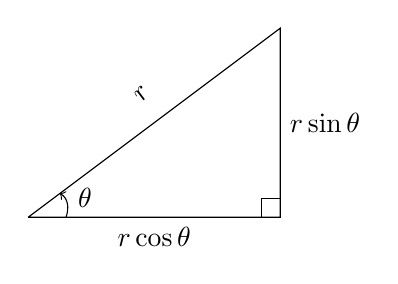
\begin{tikzpicture}[scale=.8]
	\draw [-] (0,0) -- (4,0) -- (4,3) -- (0,0);
	\draw [->] (.6,0) to[out=70, in=-30] (.5,.38);
	\node at (.9,.3) {$\theta$};
	\node [above,rotate=51] at (2,1.8) {$r$};
	\node [below] at (2,0) {$r \cos\theta$};
	\node [right] at (4,1.5) {$r \sin\theta$};
	\draw [-] (3.7,0) -- (3.7,.3) -- (4,.3);
	\end{tikzpicture}
\end{center}
Heraf følger at cosinus og sinus er forholdet mellem to længder i den
retvinklede trekant:
\begin{align*}
&\cos \theta = \frac{\text{hosliggende side}}{\text{hypotenusen}}\\
&\sin \theta = \frac{\text{modstående side}}{\text{hypotenusen}}
\end{align*}
Vi definerer også en funktion kaldet tangens:
\[
\tan \theta = \frac{\sin\theta}{\cos\theta}
= \frac{\text{modstående side}}{\text{hosliggende side}}
\]
Hvis vi sætter $r=1$ får vi fra Pythagoras' sætning at
\begin{equation*}
\cos^2 \theta + \sin^2 \theta = 1 \; ,
\end{equation*}
hvor vi har brugt notationen $\cos^2 \theta = (\cos\theta)^2$ og
$\sin^2 \theta = (\sin\theta)^2$.

\section{Differentialregning}
En bil kører på vejen, og dens position betegnes $x$. Fordi bilen
bevæger sig, ændrer dens position sig med tiden. Hvis vi lader $t$
betegne tiden, så er bilens position en \emph{funktion} af tiden, og
vi skriver $x(t)$. Vi siger også, at $x$ \emph{afhænger} af $t$. Nogle
gange er vi dovne og nøjes med at skrive $x$ i stedet for $x(t)$, men
vi husker på, at $x$ er en funktion af $t$. Måske er vi interesseret i
bilens hastighed $v$, hvilket er ændringen i position pr. ændringen i
tid. Hvis bilens position ændrer sig meget i løbet af kort tid, så er
bilens hastighed stor. Med andre ord er hastigheden til et bestemt
tidspunkt $t$ altså givet som hældningen af grafen for $x(t)$, og
hastigheden er altså selv en funktion af tiden, $v(t)$. Nedenfor ses
et eksempel, hvor bilen kører baglens for $t<5$ s, standser i $t=5$ s,
og kører fremad for $t>5$ s, hvorefter den kører hurtigere og
hurtigere som $v(t)$ vokser.

\begin{center}
	\begin{tikzpicture}
	\begin{scope}[shift={(0,0)}]
	\draw [->] (-.1,0) -- (3.3,0);
	\node [right] at (3.3,0) {$t$};
	\draw [->] (0,-.1) -- (0,2.5);
	\node [above] at (0,2.5) {$x(t)$};
	\draw [blue, domain=-.3:3.3, samples=100]
	% plot (\x, {.8+1.1*cos((\x + .56) r)*cos((3*\x) r)});
	plot (\x, {1/2*\x^2 - \x + 1/3});
	\node [left] at (-.1,0) {$0$};
	\draw (-.1,2) -- (.1,2);
	\node [left] at (-.1,2) {$2$ m};
	\node [below] at (0,-.1) {$0$};
	\draw (2,-.1) -- (2,.1);
	\node [below] at (2,-.1) {$10$ s};
	\end{scope}
	% 
	\begin{scope}[shift={(6,0)}]
	\draw [->] (-.1,0) -- (3.3,0);
	\node [right] at (3.3,0) {$t$};
	\draw [->] (0,-.1) -- (0,2.5);
	\node [above] at (0,2.5) {$v(t)$};
	\draw [blue, domain=-.3:3.3, samples=100]
	% plot (\x, {.8+1.1*cos((\x + .56) r)*cos((3*\x) r)});
	plot (\x, {\x - 1});
	\node [left] at (-.1,0) {$0$};
	\draw (-.1,2) -- (.1,2);
	\node [left] at (-.1,2) {$2$ m/s};
	\node [below] at (0,-.1) {$0$};
	\draw (2,-.1) -- (2,.1);
	\node [below] at (2,-.1) {$10$ s};
	\end{scope}
	\end{tikzpicture}
\end{center}

\subsection{Notation for Differentialkvotienter}
Differentialregning går ud på at beregne hældningen af en graf. Som
allerede illustreret med den kørende bil, så er dette yderst relevant
i fysik. En stor del af fysik har at gøre med hvordan noget ændrer
sig, når man ændrer et eller andet, f.eks. hvordan positionen ændrer
sig, når tiden ændrer sig. Tit afhænger fysiske størrelser af mere end
én variabel, men for at illustrer de grundlæggende principper ved differentiering starter vi med at kigge på funktioner af kun en variable, altså $f(x)$. Hældningen for $f$ mht. $x$ betegnes
\begin{align*}
\dif{x}{}f(x)
\qquad
\text{eller}
\qquad
\dif{x}{}f
\qquad
\text{eller blot}
\qquad
\dif{x}{f} \; ,
\end{align*}
og $\dif{x}{f}$ er en funktion af $x$, der kaldes \emph{differentialkvotienten} (eller \emph{den afledte}) af $f$ mht. $x$. Når vi beregner differentialkvotienten
siger vi, at vi \emph{differentierer} (eller \emph{afleder})
funktionen $f$ mht. $x$. Du har måske allerede stødt på dette, men
brugt mærke-notationen i stedet:
\begin{align*}
\dif{x}{f} = f'(x) \; .
\end{align*}
Mærke-notationen $f'(x)$ er uheldig, fordi den kun kan anvendes for
funktioner af én variabel; hvis funktionen afhænger af to variable,
hvilken én henviser mærket så til? Da $\dif{x}{f}$ også er en funktion,
kan vi differentiere den igen, hvilket giver
\begin{align*}
\dif{x}{} \left(\dif{x}{f}\right)
= \dif{x}{} \dif{x}{f}
= \dif[2]{x}{f}
\end{align*}
I det særlige tilfælde, hvor vi differentierer en funktion mht. tiden
$t$, så bruger vi tit en særlig prik-notation:
\begin{align*}
\dif{t}{f} = \dt{f}
\qquad
\text{og}
\qquad
\dif{t}{} \dif{t}{f} = \dif[2]{t}{f} = \ddt{f} \; .
\end{align*}
\textsl{Sidebemærkning:} Hvis man vil, kan man tænke på $\dif{x}{}$ som
en operator, der opererer på funktionen $f$. Når vi ganger operatoren
$\dif{x}{}$ på $f$ fra venstre, vil dens operation være at finde
hældningen af $f$ mht. $x$. I sig selv giver $\dif{x}{}$ ikke så meget
mening, men når den får lov til at operere på en funktion $f$, så får
vi en ny funktion, $\dif{x}{f}$.

\subsection{Regneregler}
Vi skal ikke gå i detaljer med, hvordan man matematisk finder
differentialkvotienter. Derimod vil vi postulere en række regneregler,
og dem skal vi bruge til at regne differentialkvotienten ud for en
masse funktioner. Nedenfor er $f$ og $g$ to funktioner af $x$, og $a$ er en
konstant (dvs. afhænger ikke af $x$).

\begin{enumerate}
	\item\label{itm:d-skalering} \textbf{Konstant skalering.}\\
	Hvis $a$ er en konstant kan den trækkes udenfor differentiationen.
	\[
	\dif{x}{}(a f) = a  \dif{x}{f} \; .
	\]
	\item\label{itm:d-sum} \textbf{Sum.}\\
	En sum differentieres ved at differentiere hvert led.
	\[
	\dif{x}{}(f+g) = \dif{x}{f} + \dif{x}{g} \; .
	\]
	\item\label{itm:d-produkt} \textbf{Produkt.}\\
	Et produkt differentieres ved skiftevis at differentiere hver faktor.
	\[
	\dif{x}{}(f \cdot g) =
	\left(\dif{x}{f}\right) \cdot g + f \cdot \left(\dif{x}{g}\right) \; .
	\]
	\item\label{itm:d-kvotient} \textbf{Kvotient.}\\
	En kvotient differentieres på følgende vis.
	\[
	\dif{x}{} \left( \frac{f}{g} \right)
	= \frac{\left(\dif{x}{f}\right)
		\cdot g - f \cdot \left(\dif{x}{g}\right)}{g^2} \; .
	\]
	\item\label{itm:d-kaederegel} \textbf{Kædereglen.}\\
	En sammensat funktion, $f(g(x))$, differentieres ved at
	differentiere den indre funktion, $g(x)$, mht. $x$ og gange med den
	ydre funktion $f(g)$ differentieret mht. den indre funktion, $g$.
	\[
	\dif{x}{} f(g(x)) = \dif{x}{g} \cdot \dif{g}{f} \; .
	\]
\end{enumerate}
Med de ovenstående regler kan differentialkvotienten af enhver
funktion simplificeres, så den kan beregnes ved at kende
differentialkvotienten af nogle simplere funktioner. Nu giver vi en
liste over differentialkvotienter for en række simple funktioner.

\begin{enumerate}[resume]
	\item\label{itm:d-konstant} \textbf{Konstant.}\\
	\[
	\dif{x}{}a = 0 \; .
	\]
	\item\label{itm:d-potens} \textbf{Potensfunktion.}\\
	\[
	\dif{x}{} x^a = a x^{a-1} \; .
	\]
	Specielt gælder der at
	\begin{align*}
	&\dif{x}{}x = 1 &&(a=1)\\
	&\dif{x}{}x^2 = 2 x &&(a=2)\\
	&\dif{x}{}x^3 = 3 x^2 &&(a=3)\\
	&\dif{x}{}\sqrt{x} = \frac{1}{2\sqrt{x}} &&(a=\tfrac{1}{2})\\
	&\dif{x}{} \frac{1}{x} = - \frac{1}{x^2} &&(a=-1)\\
	&\dif{x}{} \frac{1}{x^2} = - \frac{2}{x^3} &&(a=-2)
	\end{align*}
	Kombineret med regel 1 og 2, får man for polynomier
	\[
	\dif{x}{} (a_0 + a_1 x + a_2 x^2 + a_3 x^3 + \dots + a_n x^n)
	= a_1 + 2a_2 x + 3a_3 x^2 + \dots + na_n x^{n-1}
	\]
	Specielt for en lineær funktion og en parabel har vi
	\begin{align*}
	&\dif{ x }{} (a_0 + a_1 x) = a_1 && (n=1)\\
	&\dif{ x }{} (a_0 + a_1 x + a_2 x^2) = a_1 + 2a_2 x && (n=2)
	\end{align*}
	\item\label{itm:d-exp} \textbf{Eksponentialfunktion.}\\
	\[
	\dif{x}{}e^x = e^x \; .
	\]
	\item\label{itm:d-ln} \textbf{Naturlig logaritme.}\\
	\[
	\dif{x}{} \ln x = \frac{1}{x} \; .
	\]
	\item\label{itm:d-sin} \textbf{Sinus.}\\
	\[
	\dif{x}{} \sin x = \cos x \; .
	\]
	\item\label{itm:d-cos} \textbf{Cosinus.}\\
	\[
	\dif{x}{} \cos x = - \sin x \; .
	\]
\end{enumerate}

\subsection{Eksempel 1}
Vi vil differentiere funktionen $F(x) = (3 - x^2) e^{-x^2}$
mht. $x$. Vi starter med at betragte $F(x)$ som et produkt af to
funktioner, $3-x^2$ og $e^{-x^2}$, og bruger derfor regel 3.
\[
\dif{x}{F} =
\left(\dif{x}{}(3-x^2)\right) \cdot e^{-x^2}
+ (3-x^2) \cdot \left(\dif{x}{} e^{-x^2}\right)
\]
Fra regel 8 for en parabel med $a_0 = 3$, $a_1 = 0$ og $a_2 = -1$ har vi, at
\[
\dif{x}{} (3-x^2) = -2x \; .
\]
Dernæst vil vi differentiere $e^{-x^2}$, som vi betragter som en
sammensat funktion. Regel 5 med $g(x) = -x^2$ og $f(g(x)) = e^{g(x)}$
giver, at
\[
\dif{x}{} e^{-x^2} = \dif{x}{} (-x^2) \cdot \dif{g}{} e^g
= -2x \cdot e^g
= -2x e^{-x^2} \; .
\]
Vi kan nu samle resultaterne og beregne
\[
\dif{x}{F} = (-2x) \cdot e^{-x^2} + (3-x^2) \cdot (-2x e^{-x^2})
= -2x(4 - x^2) e^{-x^2} \; .
\]

\begin{figure}[h!]
	\centering
	\begin{tikzpicture}
	\begin{scope}[shift={(0,0)}]
	\draw [->] (-3,0) -- (3,0);
	\node [right] at (3,0) {$x$};
	\draw [->] (0,-.1) -- (0,3.3);
	\node [above] at (0,3.3) {$F(x)$};
	\draw [blue, domain=-3:3, samples=300]
	plot (\x, {(3-\x*\x)*exp(-\x*\x)});
	\draw (-.1,1) -- (.1,1);
	\node [left] at (-.1,1) {$1$};
	\node [below] at (0,-.1) {$0$};
	\draw (-1,-.1) -- (-1,.1);
	\node [below] at (-1,-.1) {$-1$};
	\draw (1,-.1) -- (1,.1);
	\node [below] at (1,-.1) {$1$};
	\end{scope}
	% 
	\begin{scope}[shift={(8,0)}]
	\draw [->] (-3,0) -- (3,0);
	\node [right] at (3,0) {$x$};
	\draw [->] (0,-2.5) -- (0,3.3);
	\node [above] at (0,3.3) {$\dif{x}{F}$};
	\draw [blue, domain=-3:3, samples=300]
	plot (\x, {-2*\x*(4-\x*\x)*exp(-\x*\x)});
	\draw (-.1,1) -- (.1,1);
	\node [left] at (-.1,1) {$1$};
	\draw (-1,-.1) -- (-1,.1);
	\node [below] at (-1,-.1) {$-1$};
	\draw (1,-.1) -- (1,.1);
	\node [below] at (1,-.1) {$1$};
	\end{scope}
	\end{tikzpicture}
	\caption{$F(x)$ fra Eksempel 1 og dens afledte $\dif{x}{F}$, der
		angiver hældningen af $F(x)$.}
	\label{fig:eks1}
\end{figure}

\subsection{Funktioner af Flere Variable}
Det næste vi nu skal kigge på, er tilfældet hvor man har en funktion, der afhænger af mere end en variabel, altså $f(x,y,z,\ldots)$. Her taler man om to forskellige måder at differentiere på, der kaldes for hhv. \emph{total differentiering} og \emph{partiel differentiering}, og som skrives på to forskellige måder
\begin{align*}
\dif{x}{f} \qquad \text{total differentiering} \qquad \text{og} \qquad \pdif{x}{f} \qquad \text{partiel differentiering}
\end{align*} 
Den grundlæggende forskel på de to er, at man ved en total differentiering antager, at de andre variable kan afhænge af den variabel man differentierer i forhold til, mens man ved en partiel differentiering antager, at de andre variable er konstante, og altså ikke afhænger af den variabel man differentierer i forhold til. Det betyder specielt, at partiel differentiering fungerer på samme måde, som differentiering af funktioner af en variable, som det er introduceret ovenfor, og vi kan derfor genbruge de regneregler, som allerede er blevet gennemgået. Dette er illustreret i eksempel 2 i slutningen af afsnittet. \textbf{skriv om total afledt}.

\subsection{Eksempel 2}
Vi vil nu partielt differentiere funktionen $G(x,y) = x^2 \sin y$
mht. $x$ og mht. $y$. Vi starter med at beregne $\pdif{x}{G}$, og
derfor betragter vi $y$ som en konstant.
\[
\pdif{x}{G} = \pdif{x}{} x^2 \sin y
= \left(\pdif{x}{} x^2 \right) \sin y = 2 x \sin y \; .
\]
Nu partielt differentierer vi $G$ mht. $y$, og betragter derfor $x$ som en
konstant.
\[
\pdif{y}{G} = \pdif{x}{} x^2 \sin y
= x^2 \left(\pdif{y}{} \sin y \right) = x^2 \cos y \; .
\]





\section{Integralregning}
I det tidligere kapitel var vi interesseret i at se på hvordan en
funktion ændrer sig mht. en givet variabel, såsom tiden. Hvis vi
nu havde $v(t)$ grafen fra forrige kapitel, som ses nedenunder, og
ville finde ud af hvor langt bilen har kørt mellem tiderne
$t_1=5\, s$ og $t_2 = 12\,s$, hvordan ville vi så kunne bære os an
med det? Hvis vi overvejer hvad grafen viser os, så er det hastigheden
langs y-aksen og tiden langs x-aksen. Hvis man multiplicerer disse to
får man en afstand $x = v\cdot t$. Vi kan altså finde den afstand bilen
har bevæget sig i et givet tidsrum ved at finde arealet under funktionen,
og i dette tilfælde har vi med en trekant at gøre, hvorved det areal er
$x=\frac{1}{2}\cdot h \cdot g = \frac{1}{2} \cdot v(t_2) \cdot (t_2 - t_1)$

\begin{center}
	\begin{tikzpicture}
	\begin{scope}[shift={(6,0)}]
	\draw [->] (-.1,0) -- (3.3,0);
	\node [right] at (3.3,0) {$t$};
	\draw [->] (0,-.1) -- (0,2.5);
	\node [above] at (0,2.5) {$v(t)$};
	\draw [blue, domain=-.3:3.3, samples=100]
	% plot (\x, {.8+1.1*cos((\x + .56) r)*cos((3*\x) r)});
	plot (\x, {\x - 1});
	\node [left] at (-.1,0) {$0$};
	\draw (-.1,2) -- (.1,2);
	\node [left] at (-.1,2) {$2$ m/s};
	\node [below] at (0,-.1) {$0$};
	\draw (2,-.1) -- (2,.1);
	\node [below] at (2,-.1) {$10$ s};
	\end{scope}
	
	%Indsæt figur med areal under plot shaded
	\end{tikzpicture}
\end{center}
Hvad gør vi så hvis vi befinder os i et tilfælde hvor vores funktion ikke er
lige så "simpelt" som i det forrige tilfælde? Hvad nu hvis vores $v(t)$ var et
2-grads polynomium, hvordan ville vi så kunne finde arealet under grafen i et
givet tidsrum?

Man kunne dele tidsrummet $t_2 - t_1$ op i $n$ antal tids intervaller 
$\Delta t = \frac{t_2-t_1}{n}$, og multiplicere med funktionsværdien 
i centrum af disse $\Delta t$'er. Herved vil vi få et antal rektangler,
hvor summen af deres areal vil give os en approksimation af arealet under
grafen. Hvis vi nu øger antallet $n$ af tids intervaller, så vil vores
approksimation blive bedre.

%Indsæt polynomie med rektangler

\subsection{Notation for integralregning}
Det forrige eksempel viser en praktisk anvendelse for integralregningen,
nemlig at finde arealet under en funktion i et givet interval, eller sagt
på en måde så finder vi ændringen i funktionsværdien i et givet interval.
Herudover giver integralregningen os muligheden for at udregne de funktioner
der hører til en given differentialkvotient. Dette gør integraler utrolig
brugbare inden for alle dele af fysikken.

Der findes to former for integraler, \emph{det bestemte integrale} og \emph{det ubestemte
	integrale}. Det bestemte integrale følger samme tankegang som det forrige eksempel,
hvor vi forsøger at udregne ændringen i funktionsværdien inden for et givet interval
$a$ og $b$, og defineres som
\begin{align*}
\int_{a}^{b} f(x) dx = [F(x)]_{a}^{b} = F(b) - F(x)
\end{align*}
Her er funktionen $F(x)$ stamfunktionen til $f(x)$. $F(x)$ defineres som den funktion,
der når den differentieres, giver $f(x)$.

Det andet form for integrale er det ubestemte integrale. Når man udregner et ubestemt
integrale indsættes der intet interval $a$ og $b$, men man udregner blot stamfunktion $F(x)$,
\begin{align*}
\int f(x) dx = F(x) + C
\end{align*}
I det ubestemte tilfælde er det vigtigt at huske at tilføje en integrationskonstant til
stamfunktionen, da alle mulige løsninger til integralet skal inkluderes.

\subsection{Regneregler}
Vi skal ikke gå i detaljer med, hvordan man matematisk finder
stamfunktioner. Derimod vil vi postulere en række regneregler,
og dem skal vi bruge til at regne stamfunktioner ud for en
masse funktioner. Nedenfor er $f$ og $g$ to funktioner af $x$ og $a$ er en
konstant (dvs. afhænger ikke af $x$).

\begin{enumerate}
	\item\label{itm:d-skalering} \textbf{Konstant skalering.}\\
	Hvis $a$ er en konstant kan den trækkes udenfor integralet.
	\[
	\int(af(x))dx = a \, \int f(x) dx \; .
	\]
	\item\label{itm:d-sum} \textbf{Sum.}\\
	En sum integreres ved at integrere hvert led.
	\[
	\int(f(x)+g(x))dx = \int f(x) dx + \int g(x) dx \; .
	\]
	\item\label{itm:d-produkt} \textbf{Partiel integration.}\\
	Hvis $f(x)$ og $g(x)$ opfylder sammenhængen nedenfor,så kan 
	udtrykket forsimples ved følgende. Bemærk her at $f'(x)$ 
	notationen bruges til at betegne differentialkvotienter.
	\[
	\int f(x)\cdot g(x) dx = f(x)\cdot g(x) - \int f'(x) \cdot g(x) dx  \; .
	\]
	\item\label{itm:d-kvotient} \textbf{Substitution.}\\
	Hvis $f(x)$ og $g(x)$ befinder sig på formen $f[g(x)]\cdot g'(x)$ 
	eller kan omskrives til at være på denne form, gælder den følgende
	sammenhæng:
	\[
	\int f[g(x)]\cdot g' dx = F[g(x)] + C \; .
	\]
	På bestemt form er dette
	\[
	\int_{a}^{b} f[g(x)]\cdot g'(x)dx = \int_{g(a)}^{g(b)} f(t) dt = F[g(b)]-F[g(a)] \; .
	\]
	hvor $t=g(x)$.
\end{enumerate}

Med de ovenstående regler kan stamfunktionen af de fleste
funktion simplificeres, så den kan beregnes ved at kende
stamfunktionerne af nogle simplere funktioner. Nu giver vi en
liste over stamfunktioner for en række simple funktioner.

\begin{enumerate}[resume]
	\item\label{itm:d-konstant} \textbf{Konstant.}\\
	\[
	\int a dx = ax + C \; .
	\]
	\item\label{itm:d-potens} \textbf{Potensfunktion.}\\
	\[
	\int x^a dx = \frac{1}{a+1}\cdot x^{a+1} + C\; .
	\]
	hvor $a \neq -1$. Specielt gælder der
	\begin{align*}
	&\int x dx = \frac{1}{2} x^2 + C&&(a=1)\\
	&\int x^2 dx = \frac{1}{3} x^3 + C&&(a=2)\\
	&\int x^3 dx = \frac{1}{4} x^4 + C &&(a=3)\\
	&\int \sqrt{x} dx = \frac{2}{3} x^{\frac{3}{2}} + C &&(a=\tfrac{1}{2})\\
	&\int \frac{1}{x^2} dx = - \frac{1}{x} + C &&(a=-2)
	\end{align*}
	\item\label{itm:d-exp} \textbf{Eksponentialfunktion.}\\
	\[
	\int e^x dx = e^x + C \; .
	\]
	\item\label{itm:d-ln} \textbf{Naturlig logaritme.}\\
	\[
	\int \ln x dx = x\ln x - x + C \; .
	\]
	\item\label{itm:d-sin} \textbf{Sinus.}\\
	\[
	\int \sin x dx = -\cos x  + C\; .
	\]
	\item\label{itm:d-cos} \textbf{Cosinus.}\\
	\[
	\int \cos x dx = \sin x + C\; .
	\]
\end{enumerate}

\subsection{Eksempler}

\section{Differentialligninger} \label{sec:difflign}
En differentialligning er en ligning, hvor der indgår
differentialkvotienter af en funktion, og funktionen er den
ubekendte. Et eksempel kunne være
\[
\dif{x}{f} = -4 f(x) \; ,
\]
hvor vi løser ligningen ved at finde en funktion $f(x)$, således at
ligningen er sand. I modsætningen til almindelige ligninger, hvor de
ubekendte er tal, så er det her funktioner, der er de
ubekendte. Ligningen overfor løses af funktionen
\[
f(x) = e^{-4x} \; ,
\]
hvilket vi let kan checke ved at differentiere vha. regel 5 om sammensatte funktioner fra afsnittet om differentialregning. Sætter man $g(x) = -4x$, finder man da at:
\[
\dif{x}{f} = \dif{x}{} e^{-4x}
= \left( \dif{x}{} (-4x) \right)  \cdot \left( \dif{g}{} e^{g} \right)
= -4 e^{-4x} = -4 f(x) \; .
\]
Der er generelt ingen systematisk måde at løse differentialligninger
på, så man finder altid løsninger ved at komme med et godt
gæt. Heldigvis er det ofte de samme differentialligninger, man møder
gang på gang, og derfor er følgende liste over differentialligninger
og deres løsninger meget praktisk.

\begin{enumerate}[resume]
	\item\label{itm:d-lign1} \textbf{Førsteordensligning.}\\
	Ligningen
	\[
	\dif{x}{f} = k f(x) \; ,
	\]
	hvor $k$ er en konstant løses af
	\[
	f(x) = A e^{kx} \; ,
	\]
	hvor $A$ er en arbitrær konstant, som man kan fastsætte, hvis man
	ved, at løsningsfunktionen skal tage en bestemt værdi i et bestemt
	punkt.
	\item\label{itm:d-lign2} \textbf{Andenordensligning.}\\
	Ligningen
	\[
	\dif[2]{x}{f} = -k^2 f(x) \; ,
	\]
	hvor $k$ er en konstant løses af
	\[
	f(x) = A \sin (kx) + B \cos (kx)
	\qquad \text{og} \qquad
	f(x) = A \cos (kx + \phi) \; ,
	\]
	hvor $A$, $B$ og $\phi$ er arbitrære konstanter. De to løsninger er
	faktisk ens, så man kan selv vælge hvilken, man bruger.
\end{enumerate} 

\section{Taylorrækker} \label{sec:Taylor}
I fysikken prøver man generelt at give en så præcis beskrivelse af virkeligheden som muligt, men i mange tilfælde kan det ikke lade sig gøre at løse et givet problem eksakt. Derfor må man tit vælge enten at kigge på specialtilfælde af problemet, der kan løses, eller at finde en approksimativ løsning til problemet, som kan give noget information omkring, hvordan ens fysiske system opfører sig. Et eksempel på dette kunne fx. være et pendul, hvor man tit kan antage at vinklerne er små, hvilket giver en betydeligt simplere bevægelsesligning for pendulet. Et vigtigt redskab til dette formål er Taylorrækker, som er en måde at skrive en given funktion $f(x)$ omkring et bestemt punkt $x=a$, vha. en sum af polynomier $1,x,x^2,\ldots$ Definitionen af en funktions Taylorrække omkring punktet $x=a$ er
\begin{equation} \label{eq:TaylorInf}
f(x) = \sum\limits_{n = 0}^{\infty} \frac{f^{(n)}(a)}{n!} (x-a)^n \ .
\end{equation}
Her skal $f^{(n)}(a)$ læses som funktionen $f(x)$ differentieret $n$ gange, og derefter evalueret i punktet $a$. Denne formel er måske lidt svær at gennemskue, så vi vil derfor bruge noget tid på at give lidt intuition omkring, hvorfor formlen ser ud som den gør. Lad os derfor kigge på funktionen $f(x) = e^x$ og prøve at approksimere den omkring punktet $a = 0$. Den simpleste approksimation man kan lave, er at approksimere $f(x)$ som en konstant. Da vi gerne vil beskrive funktionen omkring punktet $a=0$, er den bedste konstante approksimation $f(x)$ selv evalueret i punktet $a$. Altså
$$f(x) \approx f(a) = e^a = e^0 = 1$$
Det næste man kan gøre er da, at tilføje en hældning til vores approksimation. Det bedste valg er hældningen af $f(x)$ i punktet $a$. Den er
$$f^{(1)}(a) = \left. \dif{x}{f(x)} \right|_{x=a} = \left. \dif{x}{} e^x \right|_{x=a} \left. e^x \right|_{x=a} = e^a = 1$$
Det giver den nye approksimation af $f(x)$
$$f(x) \approx 1 + x \ ,$$
som netop opfylder både at antage værdien og hældningen af $f(x)$ i punktet $a$. Man kan så også tilføje en krumning (ændringen i hældningen) til vores approksimation. Igen er det bedste valg krumningen af $f(x)$ i punktet $a$, hvilket giver
$$f^{(2)}(a) = \left. \dif[2]{x}{f(x)} \right|_{x=a} = \left. \dif[2]{x}{} e^x \right|_{x=a} \left. e^x \right|_{x=a} = e^a = 1$$
Den nye approksimation bliver da
$$f(x) \approx 1 +  x + \frac{1}{2} x^2 \ ,$$
hvor $\tfrac{1}{2}$ er taget med for at sikre at krumningen af approksimation er lig med krumningen af $f(x)$ i punktet $a$. Ideen herfra er da blot at tilføje flere og flere led, så den flere og flere gange differentierede af $f(x)$ og approksimationen er lig med hinanden i punktet $a$. Ideen er også illustreret på figur \ref{Taylorseries_figure}, hvor approksimationen er vist for flere og flere led, der er taget med.
\begin{figure}[h!]
	\centering
	\includegraphics[scale=0.65]{matematik/Taylorseries_figure.pdf}
	\caption{Eksempel på hvordan en Taylorapproksimation af en funktion bliver mere og mere præcis jo flere led der tages med.}
	\label{Taylorseries_figure}
\end{figure}
Som en hjælp til opgaver har vi samlet Taylorrækkerne for nogle af de mest almindelige funktioner omkring $a = 0$ i tabel \ref{Taylorseries_table}.
\begin{table}[h!]
	\centering
	\caption{Taylorrækker for forskellige funktioner omkring punktet $a=0$.}
	\label{Taylorseries_table}
	\bgroup
	\def\arraystretch{2}
	\begin{tabular}{|c|c|c|c|}
		\hline
		\textbf{Funktioner}   & $e^x$ & $\cos(x)$ & $\sin(x)$  \\ 
		\hline
		\textbf{Taylorrækker} & $\sum\limits_{n = 0}^{\infty} \frac{(x-a)^n}{n!}$ & $\sum\limits_{n=0}^{\infty} (-1)^n \frac{x^{2n}}{(2n)!} $ & $\sum\limits_{n=0}^{\infty} (-1)^n \frac{x^{2n+1}}{(2n+1)!}$  \\ \hline
	\end{tabular}
	\egroup
\end{table}

\section{Komplekse Tal}

Formålet med dette afsnit er at give en kort introduktion til komplekse tal, da de er et vigtigt redskab i store dele af fysikken. Vi vil her ikke gå i dybden med den stringente matematiske konstruktion af de komplekse tal, men i stedet fokuserer på anvendelse og forskellige specifikke egenskaber, der er relevante for de ting, som I skal arbejde med på campen.\\

Før vi definerer, hvad komplekse tal er, vil vi først kigge på den imaginære enhed $i$, som er et meget vigtigt tal i forhold til at beskrive, hvad komplekse tal er. Den imaginære enhed er defineret som følger
\begin{eqnarray}
i^2 = -1 \ ,
\end{eqnarray}
og blev oprindeligt indført som løsningen til ligningen $x^2 = -1$, der ikke kan løses med reelle tal. Men med den imaginære enhed kan man løse denne type ligning på følgende måde
$$x^2 = -1 \quad \Rightarrow \quad x^2 = i^2 \quad \Rightarrow \quad x = \pm \sqrt{i^2} = \pm i \ .$$
Det virker måske lidt underligt, sådan at indføre et nyt tal som $i$ for at løse en ligning, men det skal understreges at tallet $i$ matematisk set er lige så rigtigt som de reelle tal. Nu hvor vi har indført den imaginære enhed, er vi nu klar til at give definitionen på et komplekst tal $z$. Definitionen lyder 
\begin{equation}
z = a+ib \ ,
\label{kompleks_def}
\end{equation}  
hvor $a$ og $b$ er reelle tal, der kaldes henholdsvis realdelen og imaginærdelen af det komplekse tal $z$\footnote{At $b$ kaldes imaginærdelen skyldes, at tal på formen $ib$, hvor $b$ er et reelt tal, kaldes for imaginære tal.}.  Dette skrives ofte som $\text{Re}(z) = a$ og $\text{Im}(z) = b$. Det næste spørgsmål vi skal kigge på er, hvordan man regner med komplekse tal. Mere specifikt skal vi starte med at kigge på addition, subtraktion, multiplikation og division, da disse regneoperationer dækker langt de fleste beregninger, som involverer komplekse tal. Lad derfor $z_1 = a+ib$ og $z_2 = c+id$ være to komplekse tal, og starte med at kigge på addition og subtraktion. Dette er defineret på den naturlige måde
\begin{align}
\label{kompleks_add}
z_1+z_2 = (a+c) + i(b+d) \ , \\
\label{kompleks_sub}
z_2-z_2 = (a-c) + i(b-d) \ .
\end{align}
Man lægger/trækker altså realdelene og imaginærdelene til/fra hinanden hver for sig. Når man skal gange komplekse tal sammen, gøres det ganske som man ville forvente. Man regner blot som om, man gangede to parenteser ud
$$z_1 z_2 = (a+bi)(c+id) = ac + iad + ibc + i^2bd = (ac-bd) + i(ad+bc) \ ,$$
hvilket giver os definitionen for multiplikation af komplekse tal
\begin{equation}
\label{kompleks_mul}
z_1z_2 = (ac-bd) +i(ad+bc) \ .
\end{equation}
Endeligt er der division, som kan defineres ud fra multiplikation. Dette kan illustreres ved følgende beregning
$$\frac{z_1}{z_2} = \frac{a+ib}{c+id} = \frac{a+ib}{c+id} \cdot \frac{c-id}{c-id} = \frac{(ac+bd) + i(bc-ad)}{c^2 + d^2} = \frac{ac+bd}{c^2 + d^2} + i \frac{bc-ad}{c^2 + d^2} \ ,$$
og definitionen for division af komplekse tal kan da skrives
\begin{equation}
\label{kompleks_div}
\frac{z_1}{z_2} = \frac{ac+bd}{c^2+d^2} + i\frac{bc-ad}{c^2+d^2} \ .
\end{equation}
Nu da de grundlæggende regneregler for komplekse tal er blevet gennemgået, vil vi gå videre og kigge på nogle af de andre vigtige definition og egenskaber ved de kompleks tal. Den første af disse er det der kaldes for den komplekst konjugerede af et komplekst tal $z$, og som skrives $z^*$. Hvis vi skriver $z = a+ib$ kan den komplekst konjugerede defineres som
\begin{equation}
z^* = a - ib \ .
\end{equation}
Man finder således den komplekst konjugerede af et komplekst tal $z$ ved blot at skifte fortegn på imaginærdelen. Den næste egenskab ved komplekse tal er det der kaldes for tallets modulus, og som skrives $\abs{z}$. Definitionen af modulus er da
\begin{equation}
\abs{z} = \sqrt{a^2 + b^2} \ ,
\end{equation}
og minder altså meget om definitionen for længden af en vektor i to dimensioner. Ud fra definitionen af modulus kan man også vise følgende praktiske regneregler
\begin{align}
\abs{z} &= \abs{z^*} \ , \\
\abs{z_1 z_2} &= \abs{z_1} \abs{z_2} \ , \\
\abs{z^n} &= \abs{z}^n
\end{align}
Dette bringer os videre til normkvadratet for komplekse tal\footnote{Grunden til at det kaldes for et normkvadrat er, modulus $|z|$ også i nogle sammenhænge kaldes for normen af $z$. Her holder vi os dog til at kaldes $|z|$ for modulus og $|z|^2$ for normkvadratet.}, der er defineret som følger
\begin{equation}
\abs{z}^2 = a^2 + b^2 \ .
\end{equation}
Der er altså som sådan ikke så meget nyt ved normkvadratet i forhold til modulus, men da normkvadratet optræder typisk i fysik, er det vigtigt at nævne alligevel. Specielt er følgende lighed god at kende
\begin{equation}
\abs{z}^2 = zz^* \ ,
\end{equation} 
og kan nemt eftervises ved en hurtig beregning. Det sidste vi skal kigge på nu her er Eulers formel, som er en af de mest brugbare relationer indenfor komplekse tal. Eulers formel siger at
\begin{equation}
e^{ix} = \cos(x) + i \sin(x) \ ,
\end{equation}
hvor $x$ er et reelt tal. Dette virker nok som en lidt underlig lighed, og det er umiddelbart også svært at se, hvad en eksponentialfunktion har at gøre med cosinus og sinus. En måde at bevise denne formel på er at skrive $e^{ix}$ som sin Taylorrække, og se at denne Taylorrække er lig med summen af Taylorrækken for cosinus plus $i$ gange Taylorrækken for sinus.

\section{Vektorer}
Den simpleste måde at beskrive en vektor på, er som noget der har både en længde og en retning. I forhold til notation er der forskellige måder at skrive vektorer på, f.eks. som et bogstav med en pil over $\vec{v}$. I fysikken er der dog tradition for at skrive vektorer med fed, altså $\v{v}$, så det gør vi også her. En god måde at illustrere vektorer på er vha. en pil, som det ses på Figur \ref{vektorfig}. Denne måde at beskrive en vektor på har den fordel, at man tydeligt kan se både længden og retningen af vektoren.
\begin{figure}[h!]
	\centering
	\includegraphics[scale=0.6]{matematik/fig/vektor.pdf}
	\caption{Den sorte pil er vektoren, og der er indikeret både vektorens længde og retning. }
	\label{vektorfig}
\end{figure}
Typisk vil man dog gerne regne med vektorer, og selvom det godt kan gøres vha. en grafisk metode, er der en anden repræsentation af vektorer, som egner sig bedre til dette. Denne kaldes for \emph{komposantform} (eller \emph{matrixform})  og tager udgangspunkt i et koordinatsystem. Da man i fysikken arbejder med den virkelige verden, som jo har tre rumlige dimensioner, vil vi i resten af afsnittet bruge et 3-dimensionalt koordinatsystem, som vist på Figur \ref{koordsys}. Specielt bruges et højrehåndet koordinatsystem, hvilket betyder, at hvis man tager højre hånd og peger sin tommelfinger i $x$-retningen og sin pegefinger i $y$-retningen, så vil langefingeren vise $z$-retningen, som det også ses på Figur \ref{koordsys}.\\
Ideen med komposantformen er, at man i et koordinatsystem kan beskrive en vektor, $\v{v}$, ved at angive tre tal $v_x,  v_y,  v_z$, som angiver, hvor meget vektoren peger i hhv. $x$-, $y$-, og $z$-retningen. Disse tal kaldes for vektorens komposanter, og man skriver vektoren:
\begin{equation}
\v{v} = \xyz{v_x}{v_y}{v_z}
\end{equation}
For at finde længden af vektoren, som man skriver $\abs{\v{v}}$, på komposantform, bruges Pythagoras sætning i tre dimensioner. Man får altså at:
\begin{equation}
\abs{\v{v}} = \sqrt{v_x^2 + v_y^2 + v_z^2}
\label{length}
\end{equation} 
Til sidst er det også vigtigt at vide, hvornår to vektorer er lig med hinanden. Det er de, hvis de har både samme længde og samme retning. På komposantform kan dette skrives:
\begin{equation}
\v{v} = \v{u} \quad \quad \text{hvis} \quad \quad
\begin{matrix}
v_x = u_x \\
v_y = u_y \\
v_z = u_z \\
\end{matrix}
\end{equation}
To vektorer er altså lig med hinanden, hvis deres komposanter er ens.
\begin{figure}[h!]
	\centering
	\includegraphics[scale=0.9]{matematik/fig/koordsys}
	\caption{På billedet til venstre ses reglen for et højrehåndet koordinatsystem. På billedet til højre er der vist et højrehåndet 3-dimensionalt koordinatsystem, og der er også indtegnet en vektor, $\v{v}$, med sine tre komposanter $v_x,  v_y,  v_z$.}
	\label{koordsys}
\end{figure}

\subsection{Regneregler for Vektorer}
I dette afsnit skal vi se på, hvordan man regner med vektorer. Det første spørgsmål som man kunne stille sig selv i denne forbindelse er, om man kan lægge/trække vektorer til/fra hinanden. Det kan man godt, og det gøres ved at lægge/trække komposanterne til/fra hinanden i par. Det skrives:
\begin{equation}
\v{v} \pm \v{u} = \xyz{v_x}{v_y}{v_z} \pm \xyz{u_x}{u_y}{u_z} = \xyz{v_x \pm u_x}{v_y \pm u_y}{v_z \pm u_z}
\end{equation}
En anden ting som man kan gøre med en vektor, er at gange den med en konstant $a$. Det gøres ved at gange tallet på hver af komposanterne, altså:
\begin{equation}
a \cdot \v{v} = a \cdot \xyz{v_x}{v_y}{v_z} = \xyz{a \cdot v_x}{a \cdot v_y}{a \cdot v_z}
\end{equation}
Det næste naturlige spørgsmål er nu, om man kan gange og dividere vektorer med hinanden. Det viser sig at division af vektorer ikke er defineret, men at der til gengæld er to forskellige måder at gange vektorer sammen på, som begge kaldes for vektorprodukter.\\

Den første er \emph{skalarproduktet} (eller \emph{prikproduktet}) og kaldes sådan, fordi resultatet er en skalar (altså et tal). Skalarproduktet af to vektorer skrives $\v{v} \cdot \v{u}$ og er defineret som:
\begin{equation}
\v{v} \cdot \v{u} = \xyz{v_x}{v_y}{v_z} \cdot \xyz{u_x}{u_y}{u_z}
= v_x \cdot u_x + v_y \cdot u_y + v_z \cdot u_z
\end{equation} 
Man tager altså vektorenes komposanter, ganger dem sammen i par og lægger det hele sammen. Specielt kan man kigge på skalarproduktet af en vektor med sig selv, og hvis man sammenligner med udtrykket for længden af en vektor, ligning \eqref{length}, ses, at $\v{v} \cdot \v{v} = \left| \v{v} \right|^2$. Det giver os en alternativ definition på længden af en vektor; $\abs{\v{v}} = \sqrt{\v{v} \cdot \v{v}}$.\\ 
Skalarproduktet har dog også en mere geometrisk definition, som tager udgangspunkt i vektorenes længde og vinklen mellem dem. Det er her vigtigt at understrege, at når man taler om vinklen mellem to vektorer, så menes der den mindste vinkel mellem dem, når man placerer halerne af vektorene oveni hinanden, som det ses på Figur \ref{dot_cross}. Med denne definition er skalarproduktet:
\begin{equation}
\v{v} \cdot \v{u} = \abs{\v{v}} \cdot \abs{\v{u}} \cdot \cos \theta
\end{equation} 
Det andet af de to vektorprodukter er \emph{krydsproduktet}, hvor resultatet er en ny vektor. Krydsproduktet skrives $\v{v} \times \v{u}$ og er defineret:
\begin{equation}
\v{v} \times \v{u} = \xyz{v_x}{v_y}{v_z} \times \xyz{u_x}{u_y}{u_z} = \xyz{v_y \cdot u_z - v_z \cdot u_y}{v_z \cdot u_x - v_x \cdot u_z}{v_x \cdot u_y - v_y \cdot u_x}
\end{equation} 
En vigtig egenskab ved krydsproduktet, som man ikke sådan lige kan se ud af definitionen er, at den resulterende vektor, $\v{c} = \v{v} \times \v{u}$, er vinkelret på både $\v{v}$ og på $\v{u}$. Kigger man igen på Figur \ref{dot_cross}, kan man da se, at der er to muligheder for, hvilken vej vektoren $\v{c}$ kan pege, så den er vinkelret på $\v{v}$ og $\v{u}$; nemlig ind i eller ud af figuren. Der er selvfølgelig kun en af disse, som er den rigtige retning, og heldigvis er der en nem huskeregel (typisk kaldet højrehåndsreglen) til at finde den rigtige. Man tager højre hånd og peger tommelfingeren i retningen af den første vektor og peger så sin pegefinger i retningen af den anden vektor. Da vil langefingeren give retningen af den nye vektor, $\v{c}$, på samme måde som den angiver $z$-retningen i et højrehåndet koordinatsystem. Tager man eksemplet på Figur \ref{dot_cross}, vil $\v{c}$ pege ind i figuren.\\
Ligesom med skalarproduktet har krydsproduktet også en mere geometrisk fortolkning. Det gælder nemlig at størrelsen af den vektor, som man får, når man laver et krydsprodukt, kan udtrykkes vha. længden af de to vektorer som man krydser med hinanden og vinklen mellem dem. Der gælder:
\begin{equation}
\abs{\v{v} \times \v{u}} = \abs{\v{v}} \cdot \abs{\v{u}} \cdot \sin \theta 
\end{equation}

\begin{figure}[h!]
	\centering
	\includegraphics[scale=0.7]{matematik/fig/dot_cross.pdf}
	\caption{To vektorer og deres mellemliggende vinkel.}
	\label{dot_cross}
\end{figure}
Det sidste begreb er \emph{enhedsvektorer}, der er vektorer, som har en længde på 1. For at kunne kende forskel på en almindelig vektor og en enhedsvektor, bruger man en speciel notation, hvor man sætter en "hat" over vektoren, $\hatvec{v}$. Enhedsvektorer opfylder de samme regneregler som almindelige vektorer, og på den måde er der ikke meget nyt i dem. De er dog et vigtigt notationsmæssigt redskab og bruges i mange dele af fysikken. Specielt bruger man ofte enhedsvektorer, der peger langs en af de tre koordinatakser. Disse har en speciel notation og er skrevet op nedenfor:
\begin{equation}
\xhat = \xyz{1}{0}{0} \ , \quad \quad \yhat = \xyz{0}{1}{0} \ , \quad \quad \zhat = \xyz{0}{0}{1}
\end{equation}
Med disse tre enhedsvektorer kan man nu skrive enhver vektor, $\v{v}$, på følgende måde:
$$\v{v} = \xyz{v_x}{v_y}{v_z} = \xyz{v_x}{0}{0} + \xyz{0}{v_y}{0} + \xyz{0}{0}{v_z} = v_x \xhat + v_y \yhat + v_z \zhat$$
Denne metode, hvor man skriver en vektor som summen af flere andre vektorer, er vigtig at bide mærke i. Hvis en vektor, $\v{v}$, repræsenterer en fysisk størrelse, f.eks. en kraft, så vil den fysiske størrelse være uændret, om man skriver vektoren på den ene eller anden måde. Dette er praktisk, da man selv kan vælge på hvilken måde man skriver vektoren, alt efter hvilken fysisk problemstilling man prøver at løse. 